\chapter{Interface gráfica da estação base}

A interface gráfica desenvolvida para a estação base está representada nas Figuras \ref{fig:interface_estacao_base1} e \ref{fig:interface_estacao_base2}. O usuário tem acesso na janela principal aos recursos básicos, como imagem da webcam, controles de movimentação do robô e visualização do mapa.
A parte de visualização 2D do mapa (a maior área da janela principal) foi desenvolvida a partir da biblioteca do Processing. O visualizador 2D (classe \textit{Viewer2D} apresentada anteriormente) possui recursos de arraste, \textit{zoom} e rotação, desenvolvidos a partir do zero pela equipe. O usuário pode salvar e carregar os mapas criados com o robô através dos botôes do canto superior esquerdo da janela. A conexão com o robô pode ser feita rapidamente com o botão ``Conexão'', e o controle de gravação do mapa e recebimento de dados dos sensores e da webcam pode ser feito a utilizando-se dos dois botôes logo a seguir. Com o botão ``Reposicionar'', o usuário pode efetuar o reposicionamento do robô no mapa. 

O botão ``Avançado'' abre uma janela que possui recursos de configuração e utilização avançada, o que inclui alteração dos parâmetros de ajuste fino, como média móvel dos sensores IR e limiares de aceleração e velocidade angular. Além disso, está presente um recurso bastante útil que é o de salvar em um arquivo amostras dos sensores da maneira que são recebidas (sem nenhum tratamento adicional). O programa e o algoritmo de criação do mapa podem ser alterados, e essas amostras podem ser posteriormente carregadas para efetuar testes das alterações feitas. Vale ressaltar que, no decorrer do projeto, esse foi um recurso que melhorou o rendimento da equipe, pois dessa forma testes práticos com o robô não necessitavam ser repetidos continuamente para testar modificações no programa.

\begin{figure}[H]
	\centering
	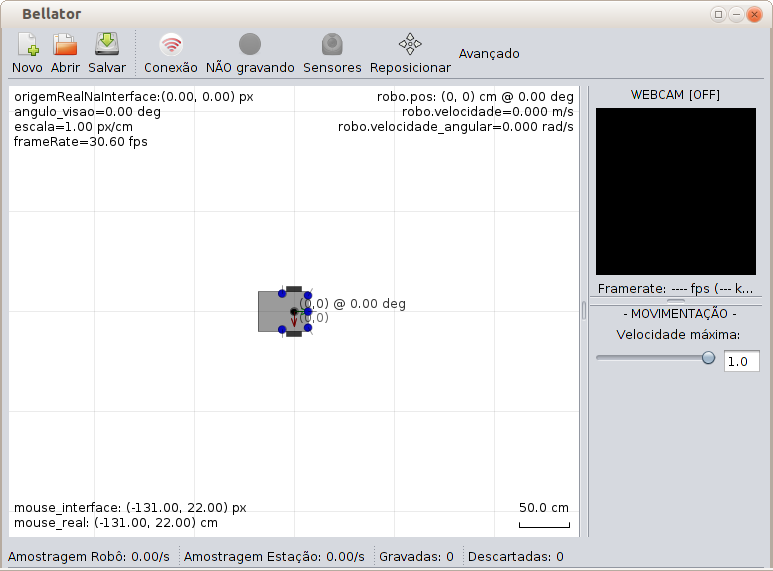
\includegraphics[width=1\textwidth]{./figuras/estacaoBase/interface_estacao_base1.png}
	\caption{Janela principal da interface gráfica da estação base.}
	\label{fig:interface_estacao_base1}
\end{figure}
\begin{figure}[H]
	\centering
	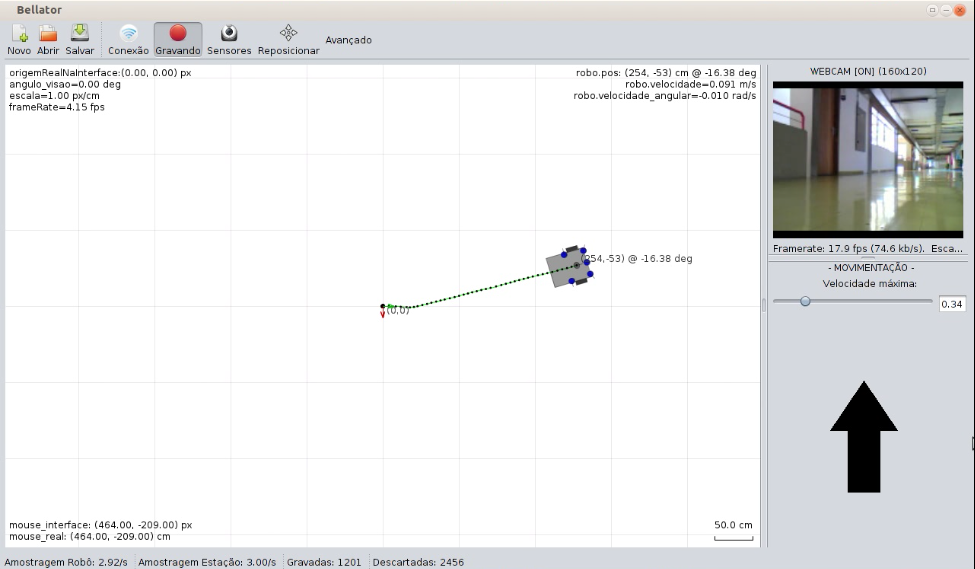
\includegraphics[width=1\textwidth]{./figuras/estacaoBase/interface_estacao_base2.png}
	\caption{Estação base em utilização na prática.}
	\label{fig:interface_estacao_base2}
\end{figure}